\pagestyle{empty}
\begin{center}
\Huge{\pack } \\
\Large{An \R~package to set, describe and analyse balanced and unbalanced trials in decentralized participatory plant breeding programmes}

~\\

\warning{Be aware that this package is under development and test: do not 100\% trust the functions!!! You're welcome to contribute. See \texttt{vignette("contribute")} for more details.}

~\\

version \versionnumber \\

~\\
\today

~\\~\\

Pierre Rivi\`ere\textsuperscript{1,2} \hspace{.5cm} 
Gaelle Van Frank\textsuperscript{2} \hspace{.5cm}
Olivier David\textsuperscript{3}  \hspace{.5cm} 
Facundo Muñoz\textsuperscript{4}
\\
~\\~\\ 
\end{center}

\vfill

\noindent\textsuperscript{1} R\'eseau Semences Paysannes, 3 avenue de la gare, F-47190 Aiguillon, France \\
\textsuperscript{2} INRA, UMR 0320, Génétique Quantitative et Evolution, Ferme du Moulon F-91190 Gif sur Yvette, France \\
\textsuperscript{3} INRA, UR 1404 Unité Mathématiques et Informatique Appliquées du Génome à l'Environnement, F-78352 Jouy-en-Josas, France \\ 
\textsuperscript{4} INRA, Centre Val de Loire, Unité Amélioration, Génétique et Physiologie Forestières, F-45075 Orléans, France \\ 
\textbf{Contact:} \href{mailto:pierre@semencespaysannes.org}{pierre@semencespaysannes.org} \\

\vfill

\noindent\textbf{Contributions:} \\
PR coordinates the package development, wrote the \texttt{R} functions and the vignette \\
GVF test the package and updated the code regarding Sections~\ref{ammi}, \ref{gge}, \ref{model_1} and \ref{model_2} \\
OD wrote the \texttt{JAGS} code and reviewed the \texttt{R} code and the vignette regarding Sections~\ref{model_1} and \ref{model_2} \\
FM reformated and improved all the code especially regarding S3 methods and reviewed and improved the vignette. \\

\vfill

\begin{center}
Copyright Réseau Semences Paysannes and Institut National de la Recherche Agronomique \\
\href{http://creativecommons.org/licenses/by-nc-sa/4.0/}{Licence creative commons BY-NC-SA 4.0} \\
\vspace{.25cm}
\href{http://creativecommons.org/licenses/by-nc-sa/4.0/}{
\includegraphics[width=.15\textwidth]{cc-by-nc-sa}}
\end{center}

\clearpage

\begin{wrapfigure}{l}{.15\textwidth}
\begin{center} \vspace{-20pt}
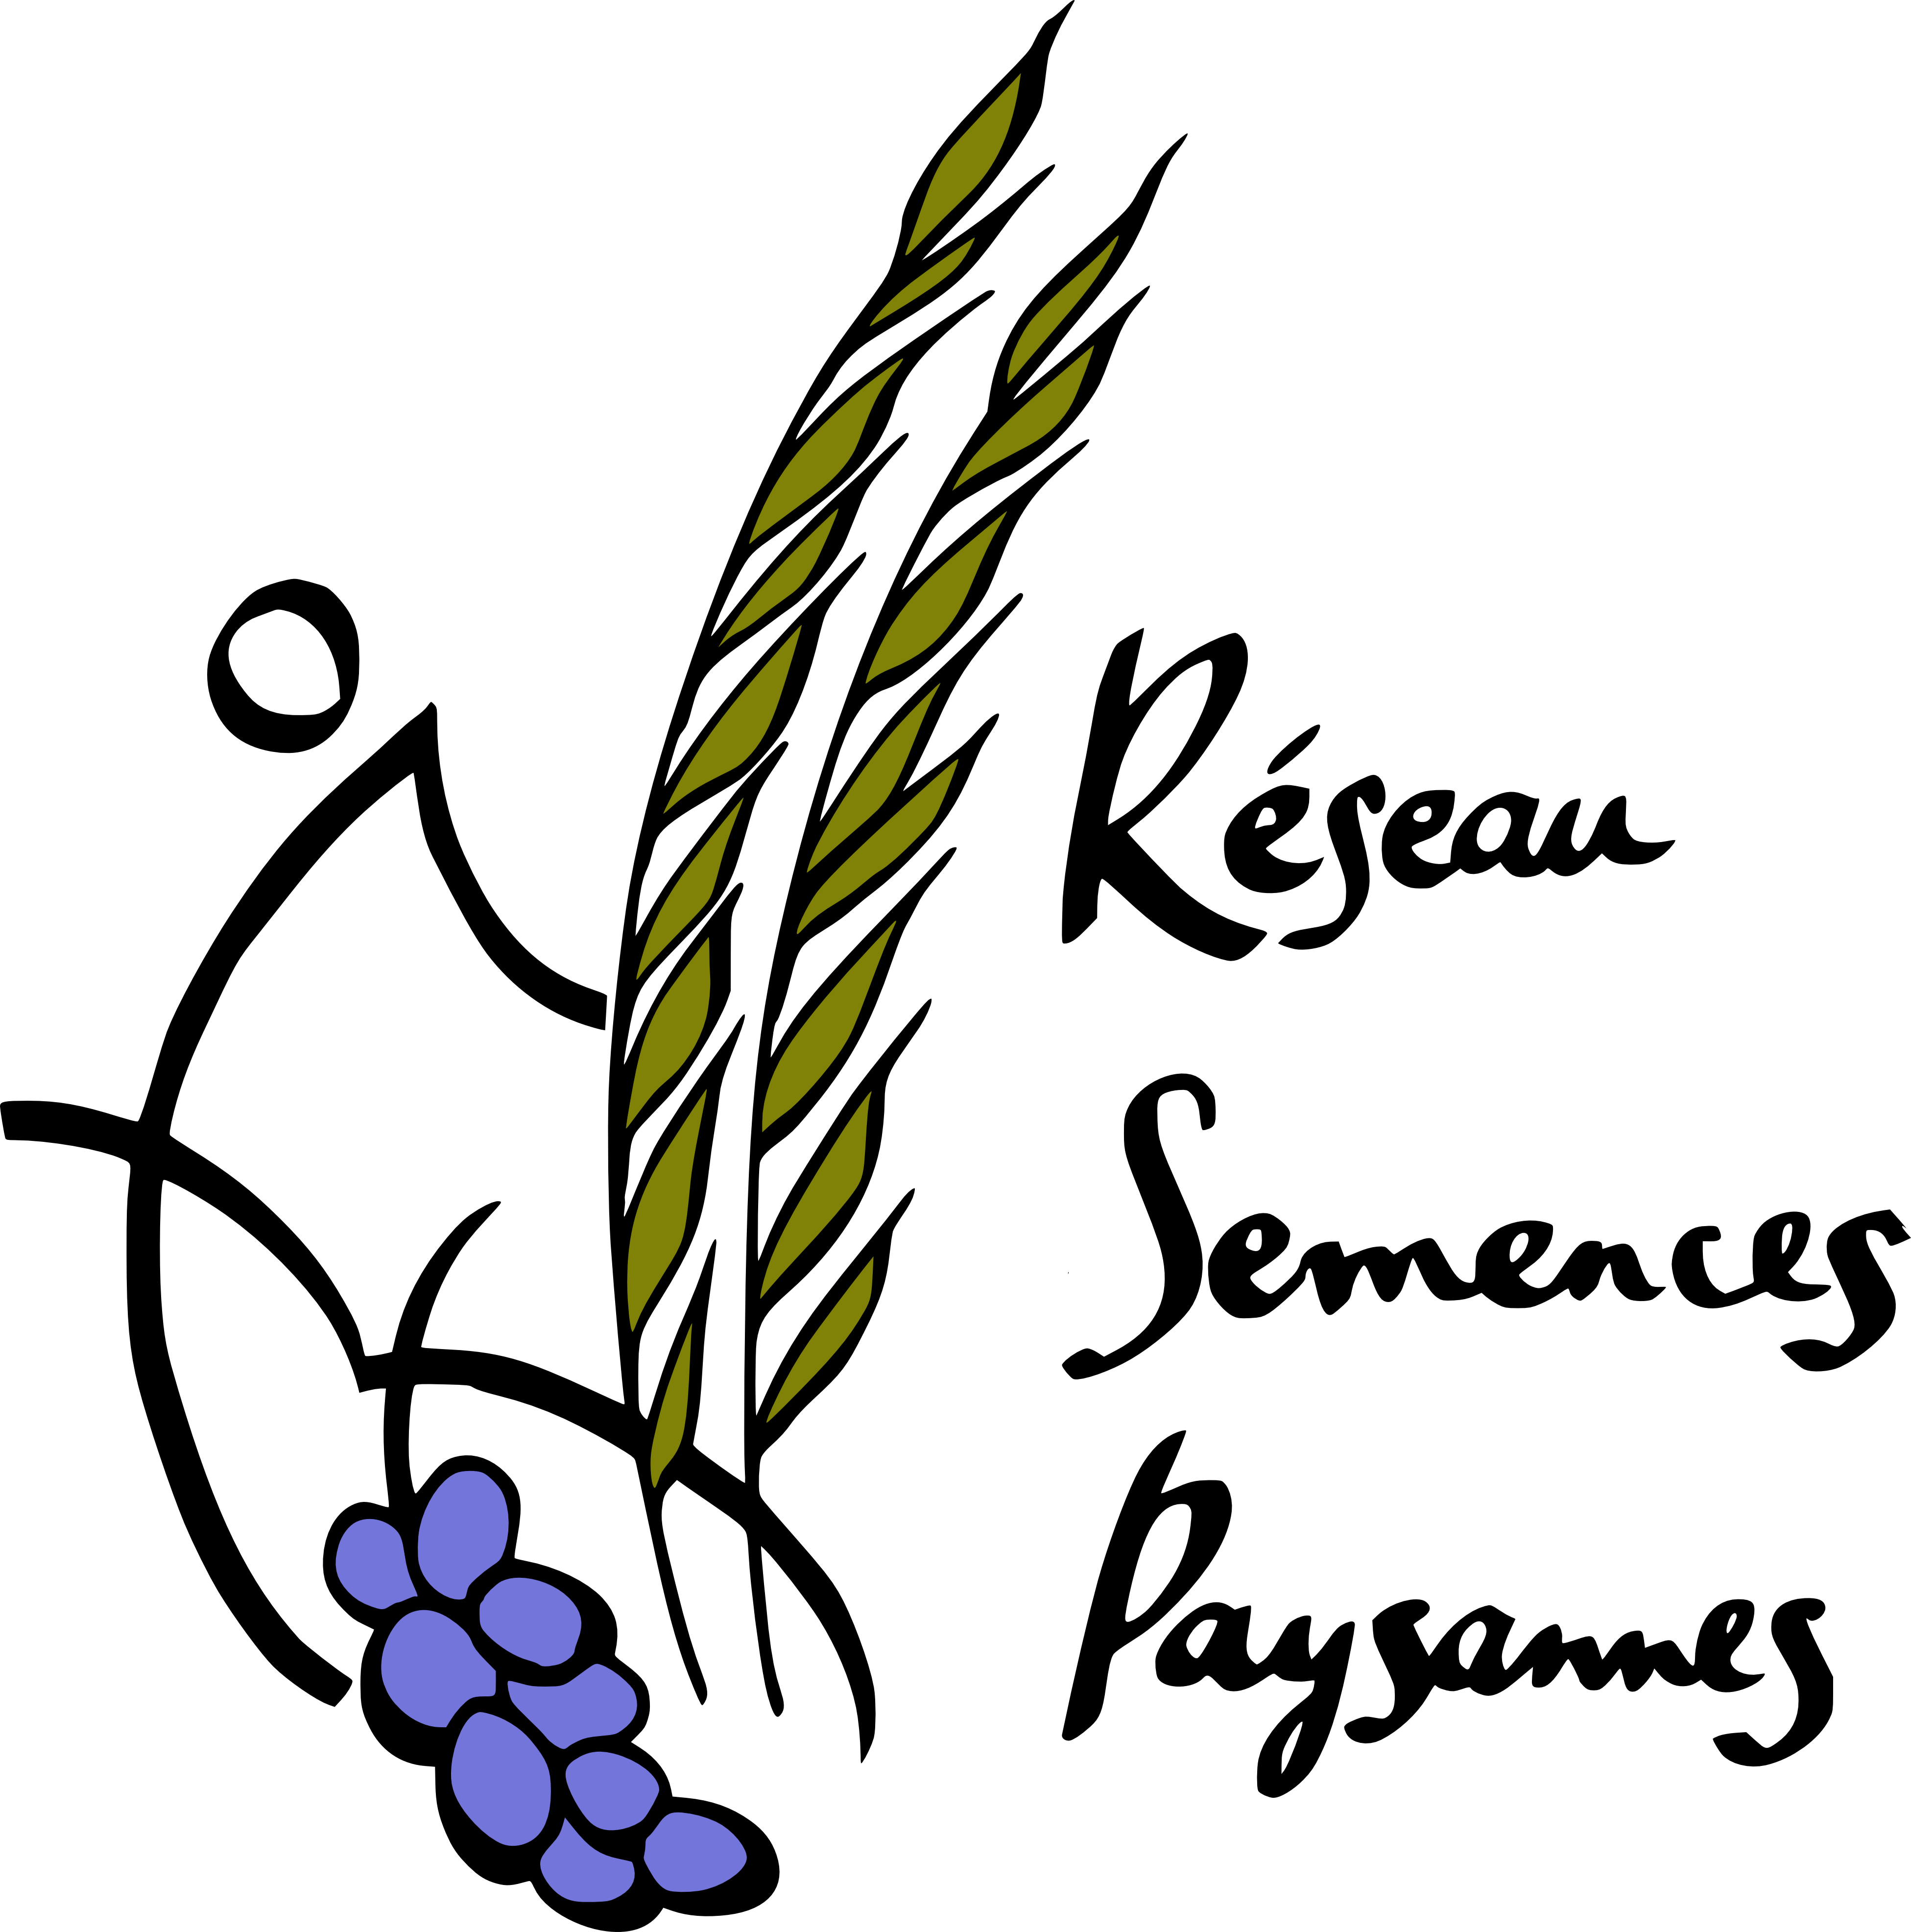
\includegraphics[width=.15\textwidth]{Logo-RSP}
\end{center} \vspace{-20pt}
\end{wrapfigure}
\noindent
Le Réseau Semences Paysannes (the French Farmers' Seeds Network (RSP)), created in 2003, brings together a great diversity of collectives and people who preserve farmers' seeds in fields, orchards, vineyards and gardens. They are involved in supporting the consolidation of local initiatives to maintain and renew cultivated biodiversity through Community Seeds Systems. Over 80 organizations have come together to promote and develop farmers' seeds, and to protect farmers' rights over their seeds. \\
\url{www.semencespaysannes.org} (in french).


\vfill

\begin{wrapfigure}{l}{.15\textwidth}
\begin{center} \vspace{-20pt}
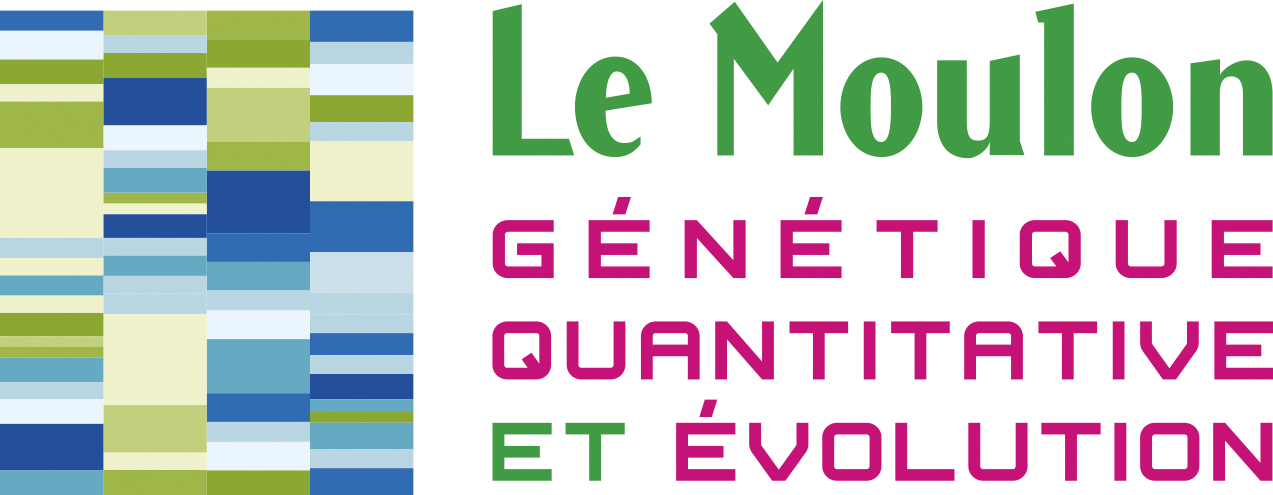
\includegraphics[width=.15\textwidth]{Logo-UMRGV}
\end{center} \vspace{-20pt}
\end{wrapfigure}
\noindent
The Diversity, Evolution and Adaptation of Populations (DEAP) team led by Isabelle Goldringer is part of INRA UMR 0320 Quantitative Genetic and Evolution.
Its work is based on the analysis of the genetic and evolutionary mechanisms underlying evolution and adaptation of crop populations.
DEAP develops strategies for on farm management of crop genetic diversity and
for plant breeding (evolutionary and/or participatory) adated to organic and low input agriculture.
Assessing the benefits of in-field genetic diversity (variety mixtures, populations) and designing
/ breeding optimized mixtures adapted to local conditions are also key research objectives.\\
\url{http://moulon.inra.fr/index.php/en/team/deap}


\vfill


\begin{wrapfigure}{l}{.15\textwidth}
\begin{center} \vspace{-20pt}

\includegraphics[width=.15\textwidth]{Logo-maiage}
\end{center} \vspace{-20pt}
\end{wrapfigure}
\noindent
The INRA UR1404 MaIAGE research laboratory gathers mathematicians, computer scientists, bioinformaticians and biologists to tackle problems coming from biology, agronomy and ecology; The addressed questions may concern processes at very different levels: molecular, cellular or multicellular, individual, populations, ecosystems oy landscapes. 
MaIAGE develops original methods in mathematics, statistics and computer science which are generic or driven by specific biological problems. A particular attention is paid to develop and make available softwares, databases, ontologies and web services so that biologists can use them easily to analyze their data or to mine the scientific literature.\\
\url{http://maiage.jouy.inra.fr/?q=en/home}



\newpage

\tableofcontents

\vfill

\begin{center}
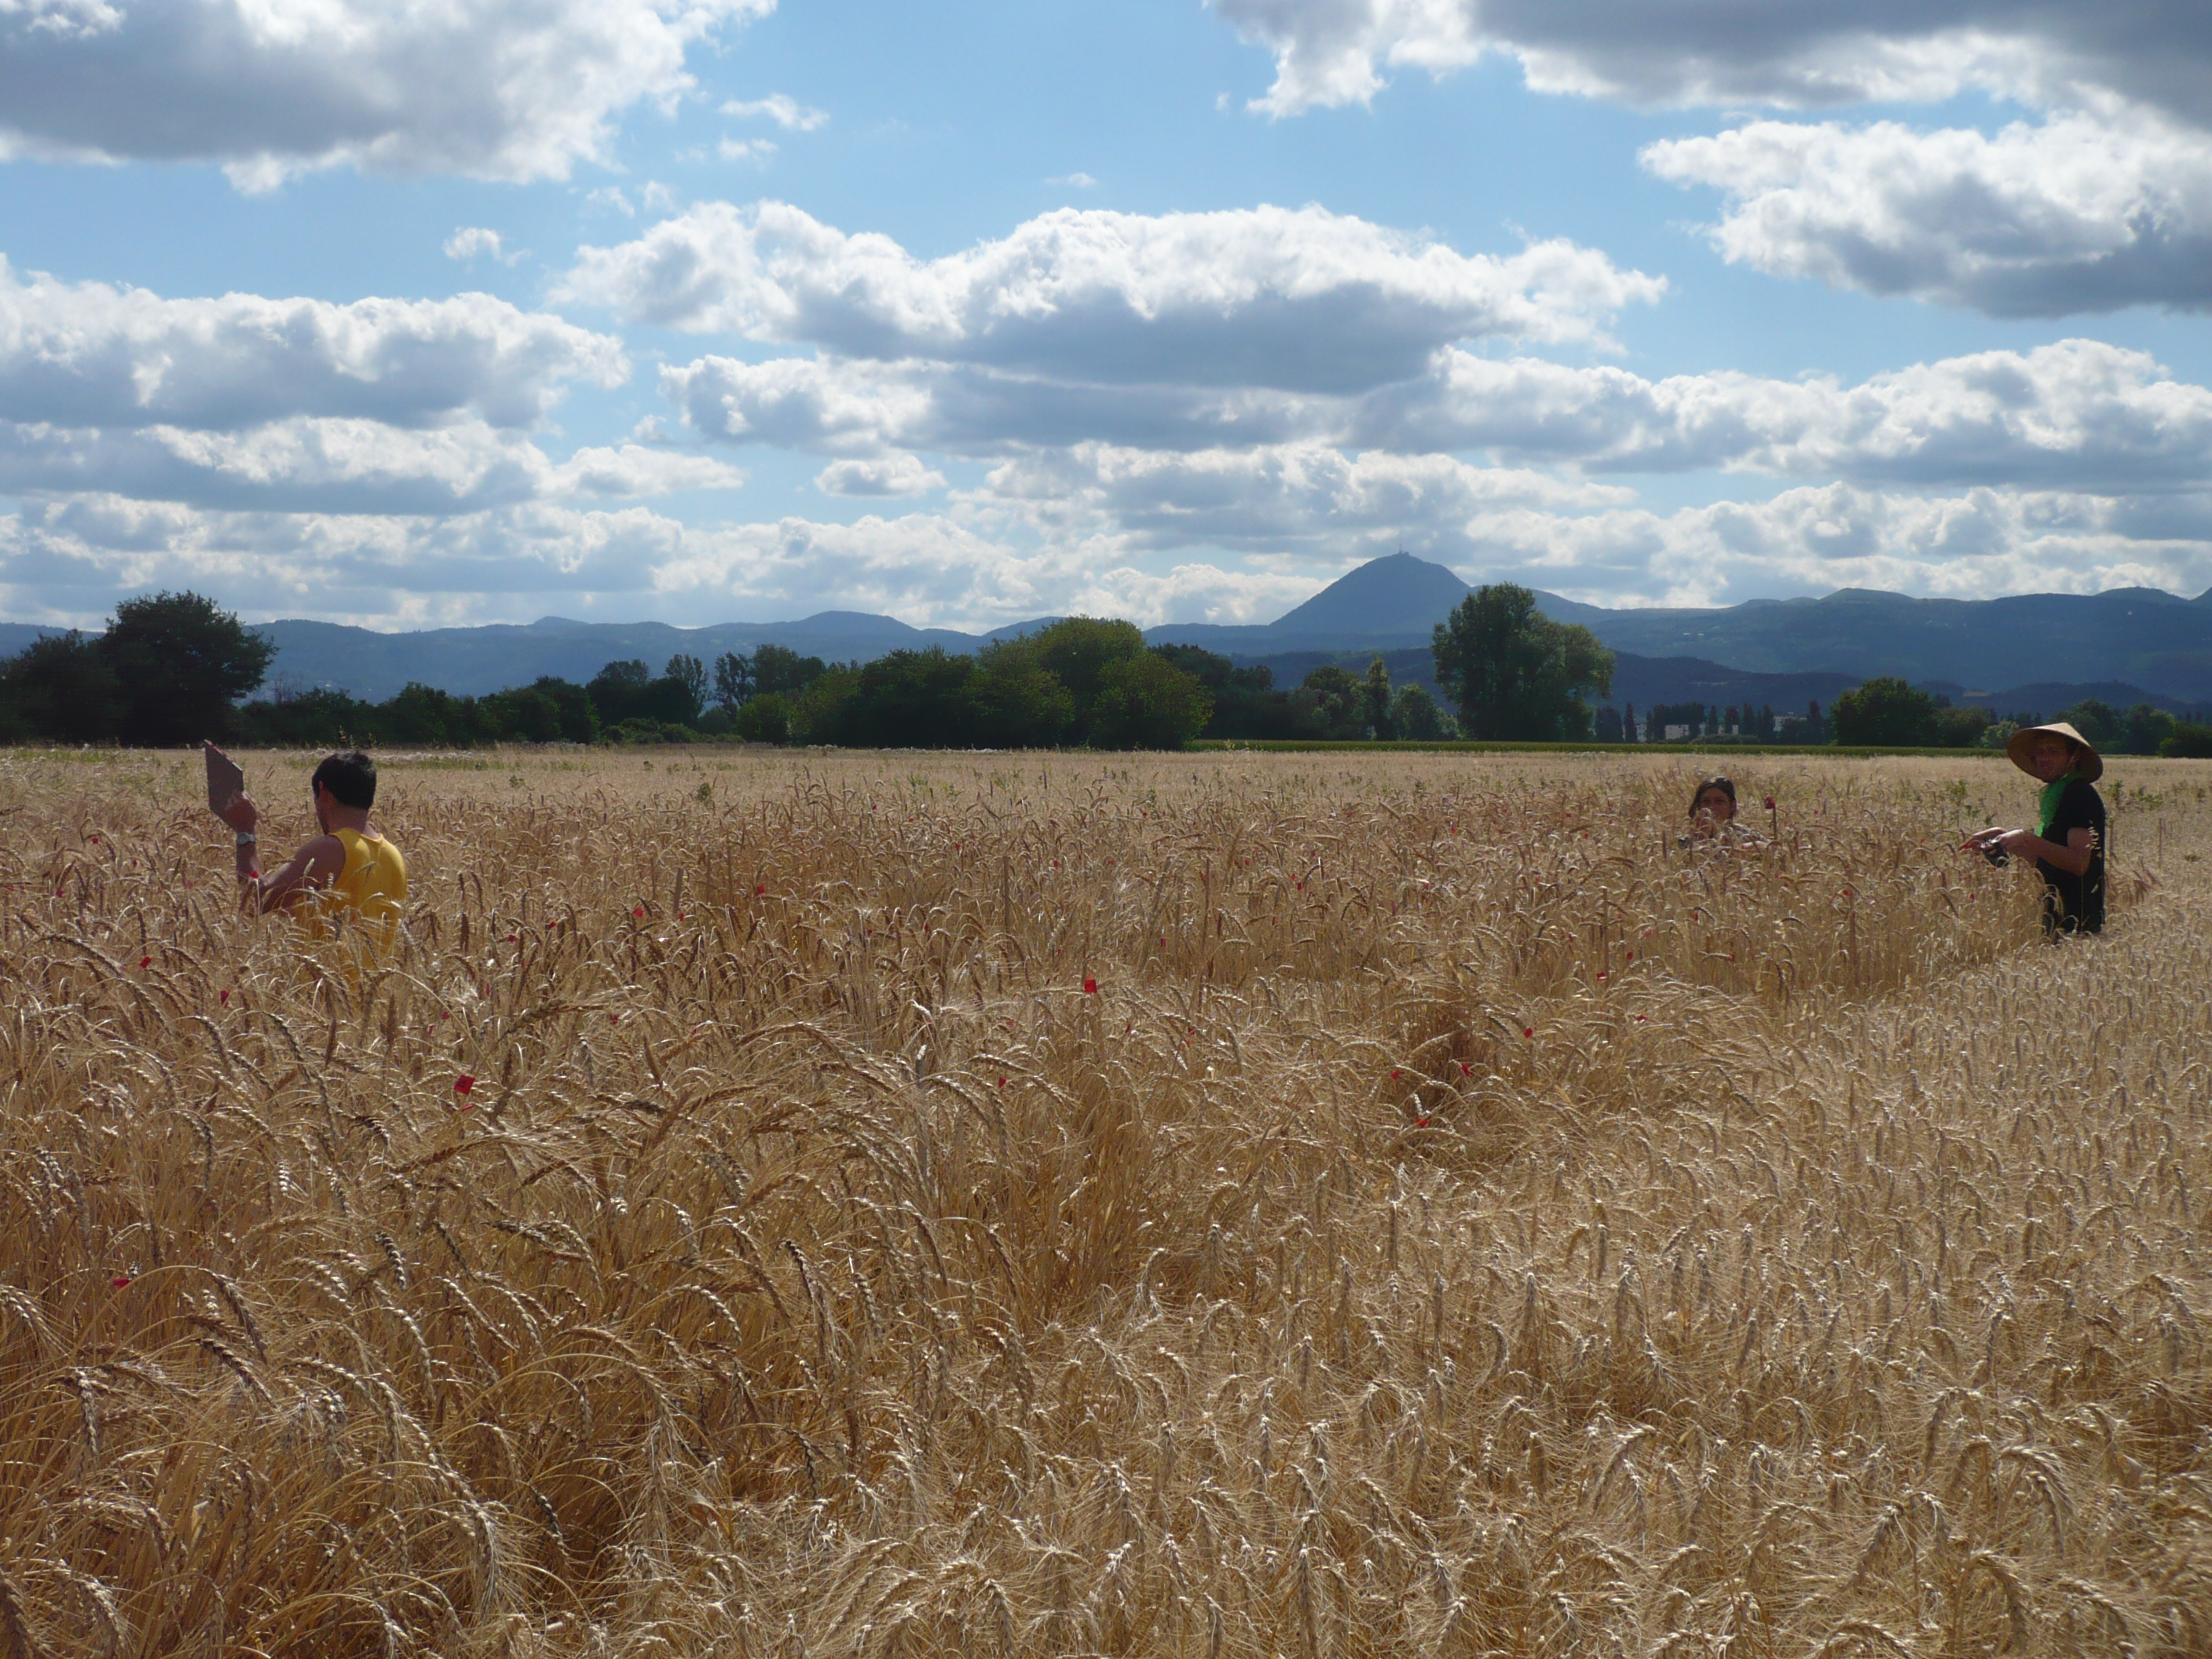
\includegraphics[width=.8\textwidth]{wheat} \\
Wheat trials on farm within our participatory plant breeding programme, summer 2012, Auvergne, France. \\
CC-BY-NC-SA. Pierre Rivière.
\end{center}

\newpage
\pagestyle{plain}
